\chapter{Appendices}

\section{Model Deployment}

\begin{figure}
    \centering
    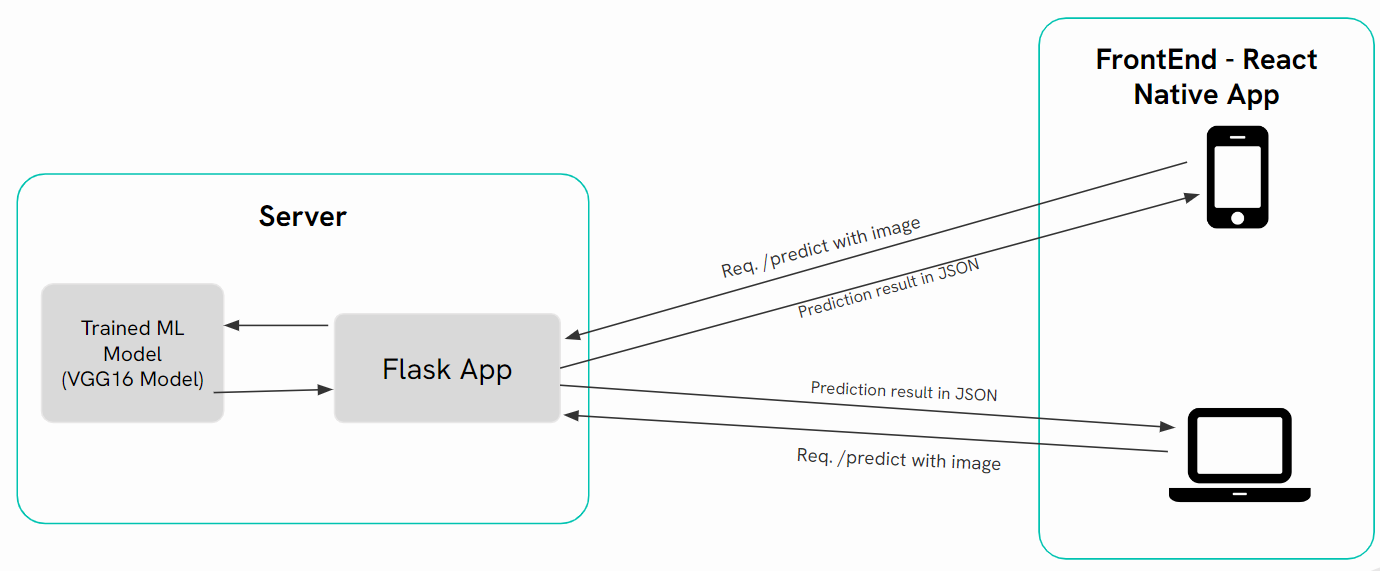
\includegraphics[width=1\linewidth]{graphics//chapter9/model deployment.png}
    \caption{ML Model Deployment Pipeline}
    \label{fig:model-deployment}
\end{figure}
% \FloatBarrier

\section{Application Prototype}
% \begin{figure}
%     \centering
%     \begin{sideways} 
%         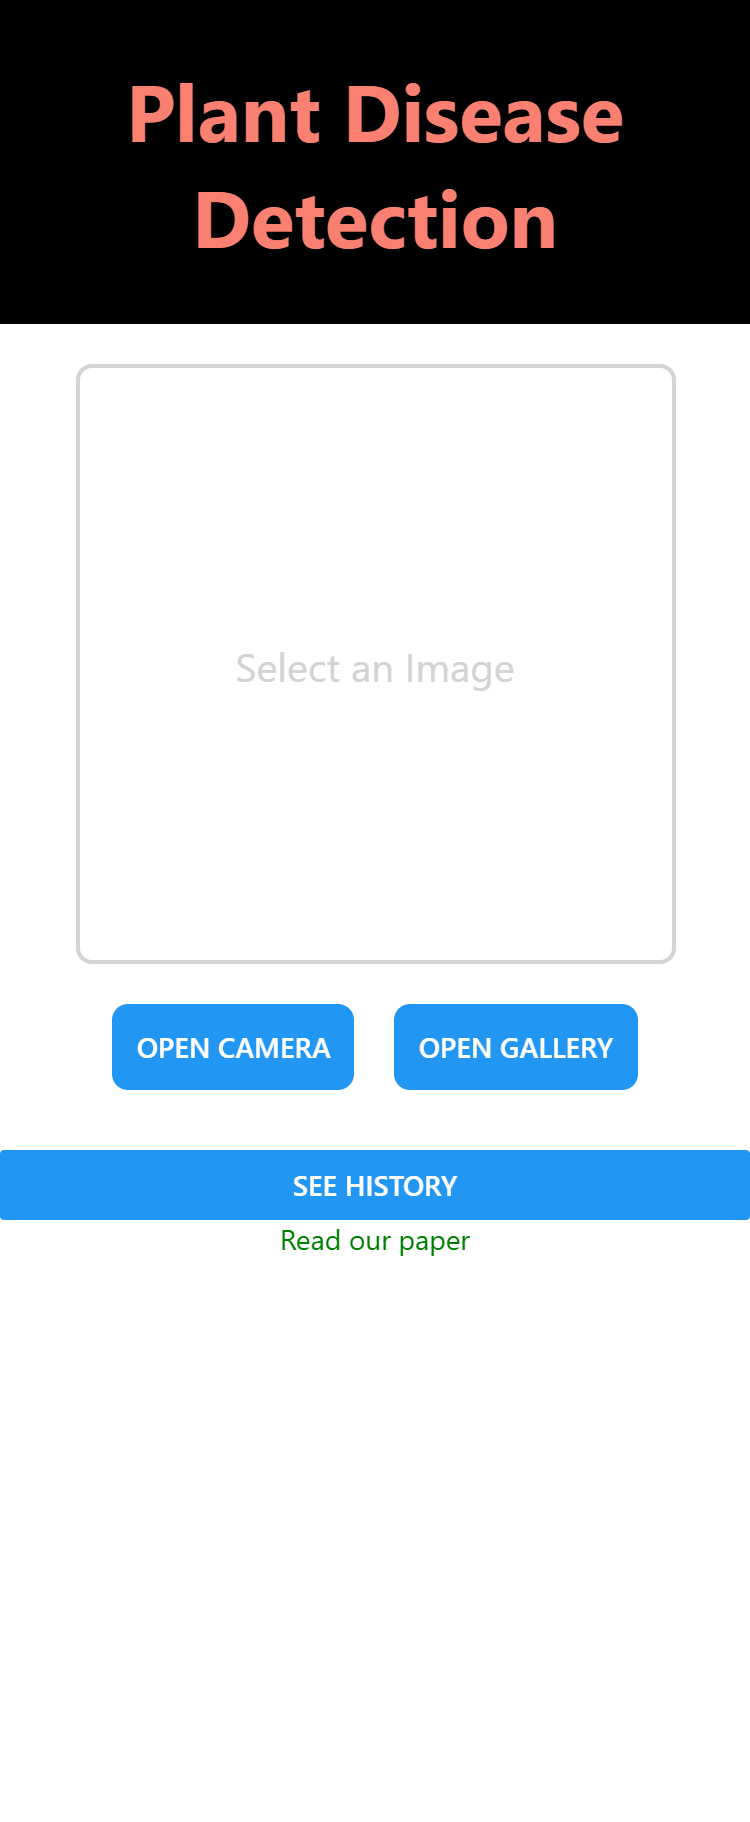
\includegraphics[height=\linewidth]{graphics//chapter9/app-0.png}
%         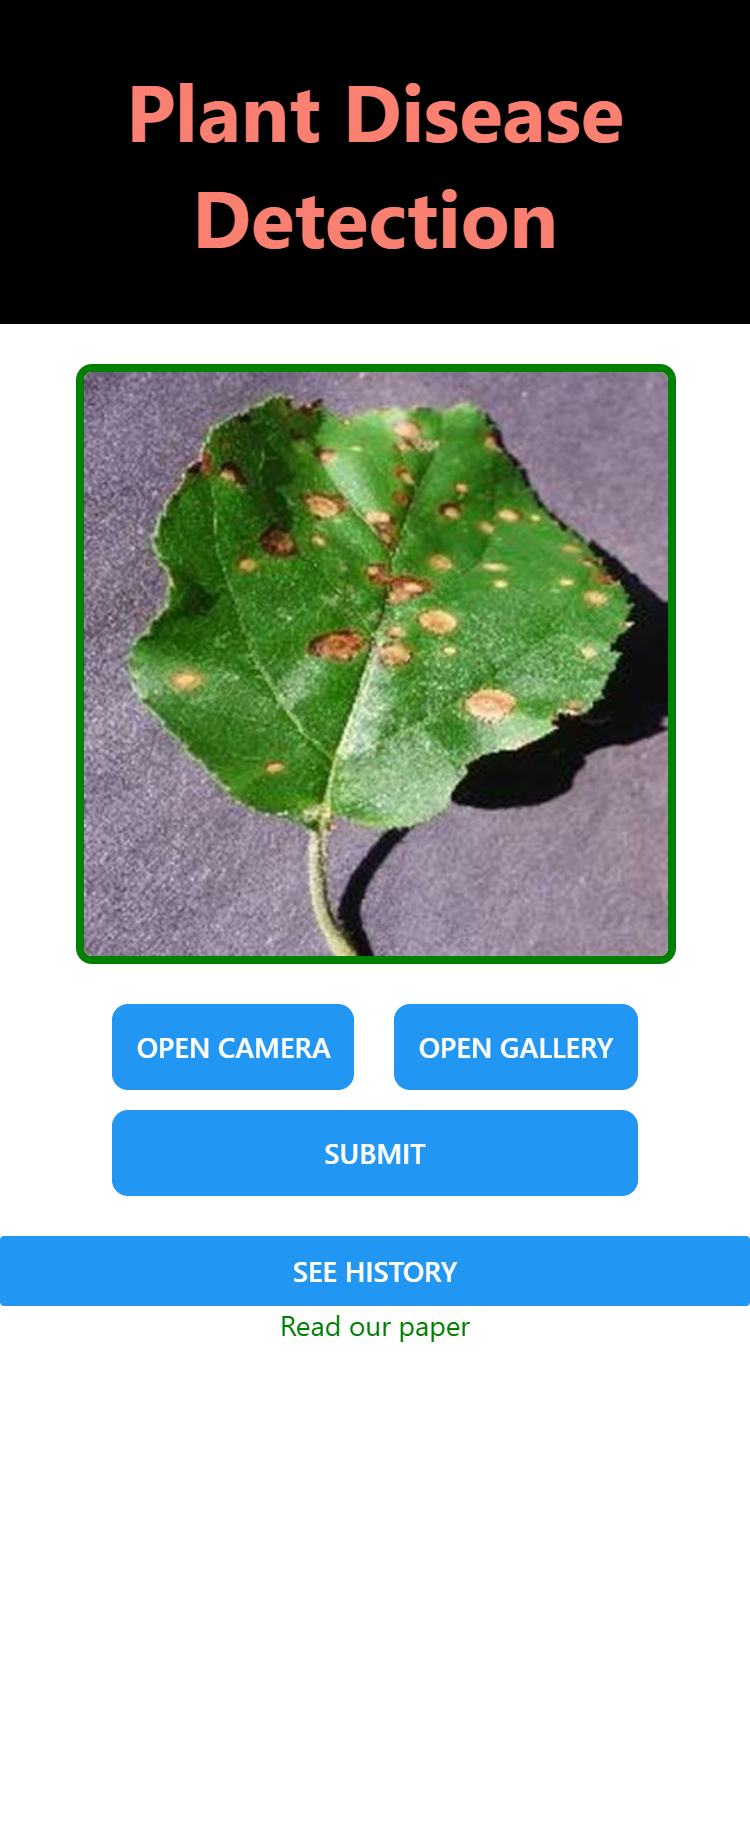
\includegraphics[height=\linewidth]{graphics//chapter9/app-1.png}
%         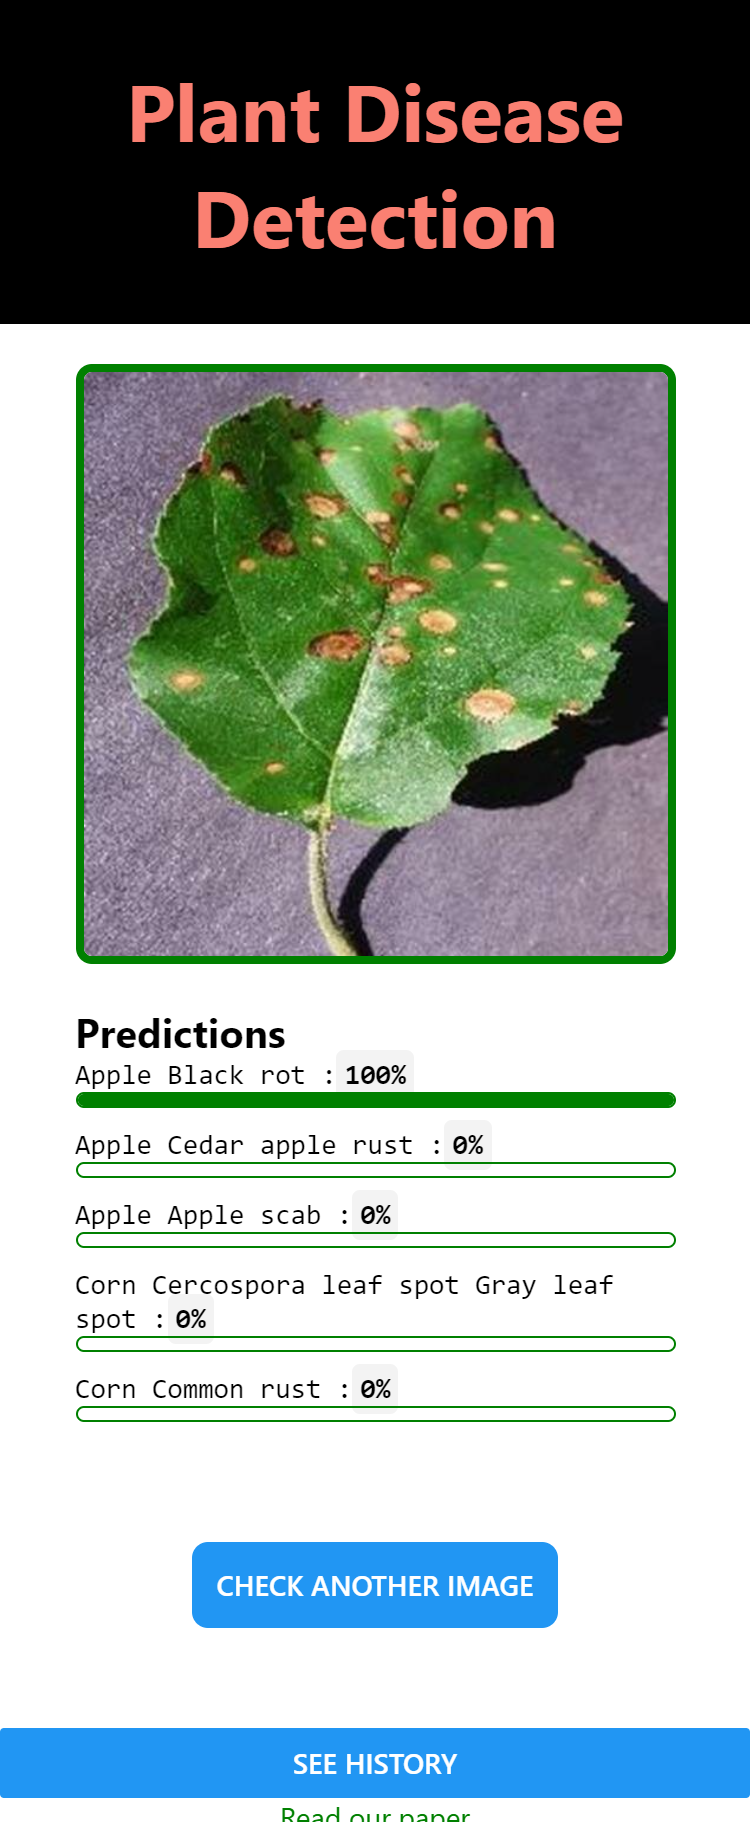
\includegraphics[height=\linewidth]{graphics//chapter9/app-3.png}
%     \end{sideways}
%     \caption{App Image Select Page} 
%     \label{fig:app-1}
% \end{figure}

\begin{sidewaysfigure} % This rotates the entire figure including the caption
    \centering
        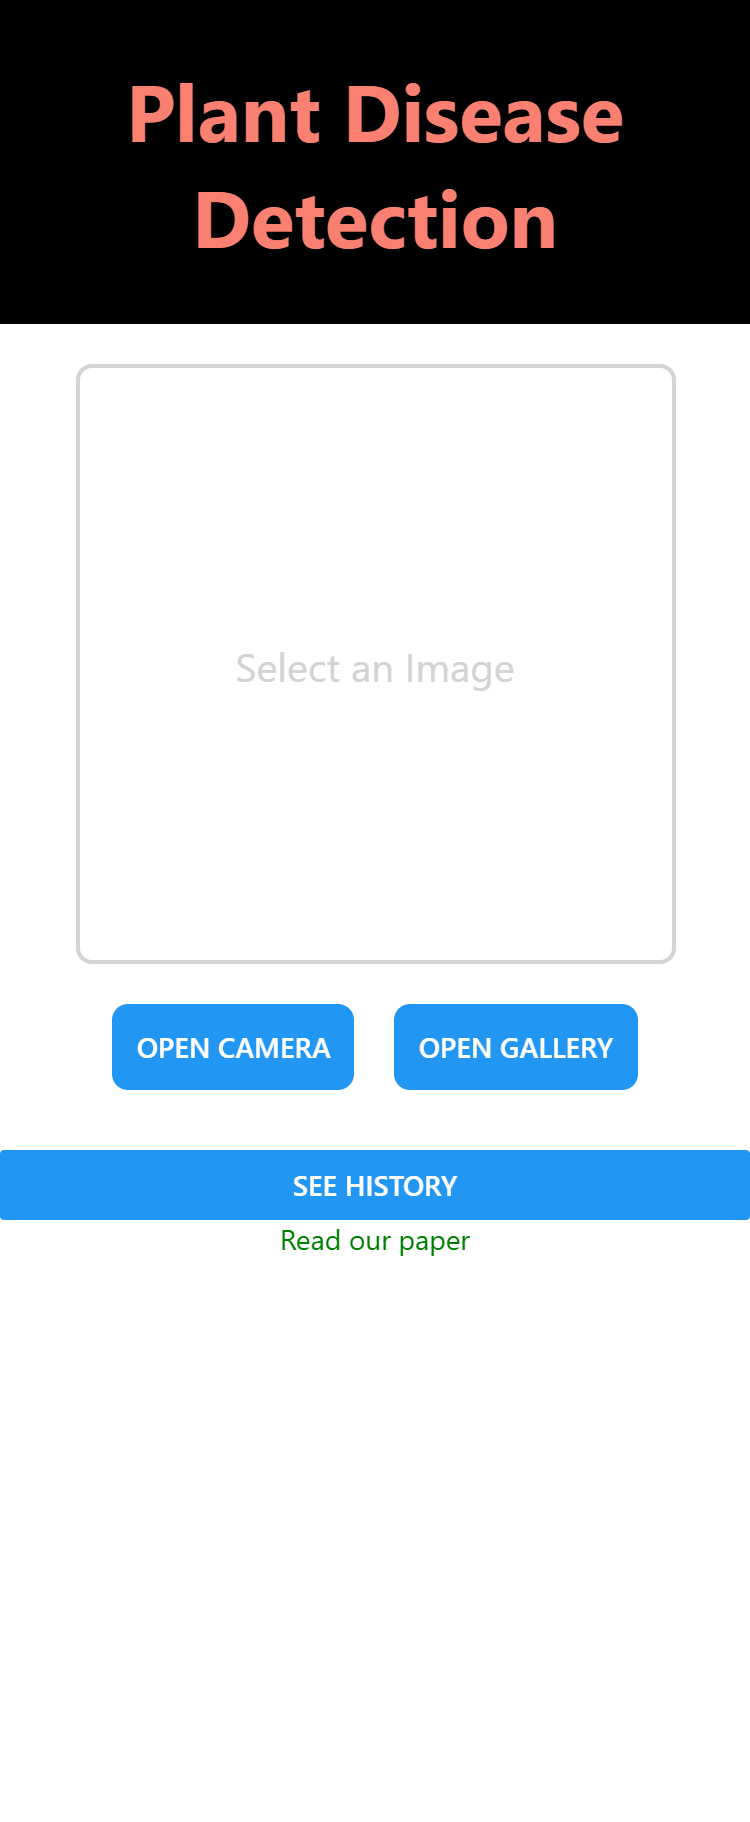
\includegraphics[height=.8\linewidth]{graphics//chapter9/app-0.png}
        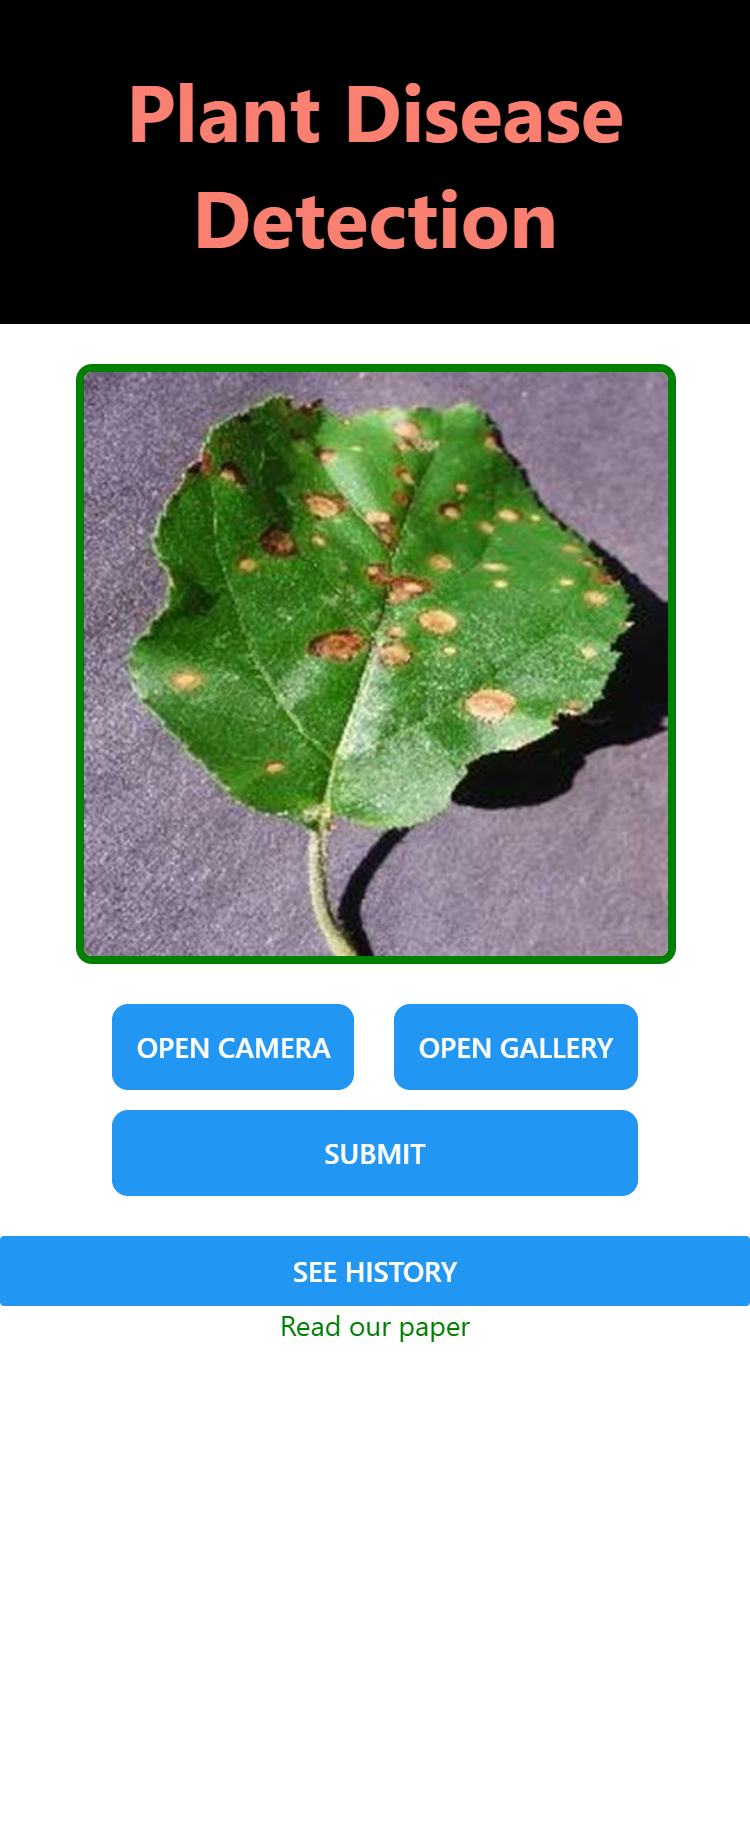
\includegraphics[height=.8\linewidth]{graphics//chapter9/app-1.png}
        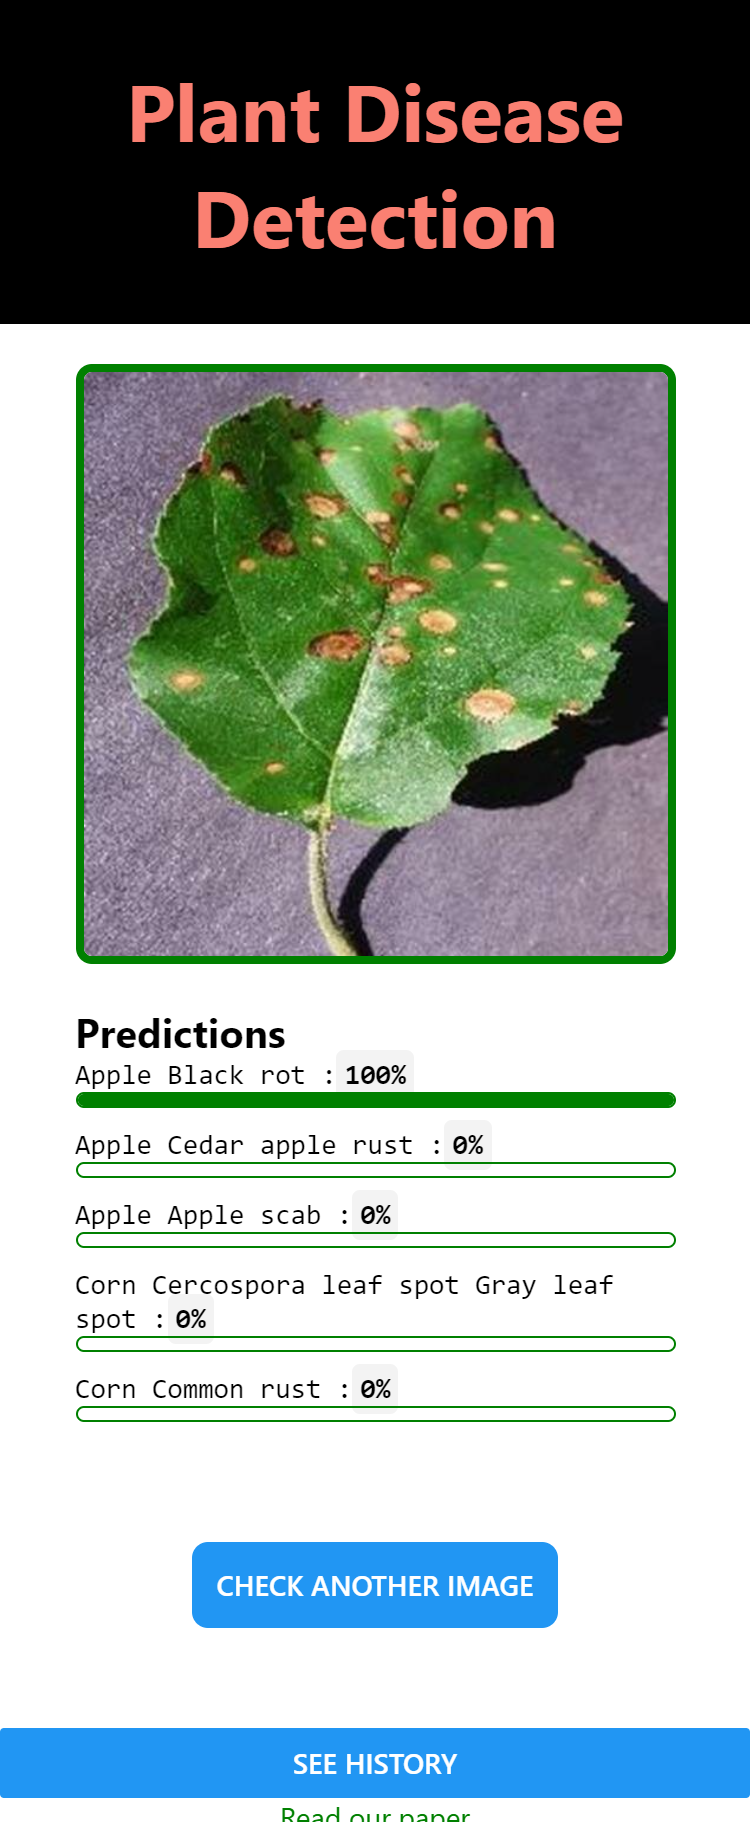
\includegraphics[height=.8\linewidth]{graphics//chapter9/app-3.png}
    \caption{App prototype, From left to right: App Main Page, App Image Select Page and App Image Result Page}
    \label{fig:app-1}
\end{sidewaysfigure}


\FloatBarrier
\section{Additional Table}


\begin{table}[h]
    \centering
    \begin{tabular}{|c|l|}
        \hline
        \textbf{Class ID} & \textbf{Class Names} \\
        \hline
        0 & Apple\_\_Apple\_scab \\
        \hline
        1 & Apple\_\_Black\_rot \\
        \hline
        2 & Apple\_\_Cedar\_apple\_rust \\
        \hline
        3 & Apple\_\_healthy \\
        \hline
        4 & Blueberry\_\_healthy \\
        \hline
        5 & Cherry\_\_healthy \\
        \hline
        6 & Cherry\_\_Powdery\_mildew \\
        \hline
        7 & Corn\_\_Cercospora\_leaf\_spot\_Gray\_leaf\_spot \\
        \hline
        8 & Corn\_\_Common\_rust \\
        \hline
        9 & Corn\_\_healthy \\
        \hline
        10 & Corn\_\_Northern\_Leaf\_Blight \\
        \hline
    \end{tabular}
    \caption{Total Classes Number: 11}
    \label{tab:class_table}
\end{table}

% MobileNetV2

\begin{table}[h]
    \centering
    \begin{tabular}{cccccc}
        \toprule
        \textbf{Class ID} & \textbf{Precision} & \textbf{Recall} & \textbf{F1-score} & \textbf{Support} \\
        \midrule
        0 & 1.00 & 1.00 & 1.00 & 63 \\
        1 & 1.00 & 1.00 & 1.00 & 62 \\
        2 & 0.96 & 1.00 & 0.98 & 26 \\
        3 & 1.00 & 1.00 & 1.00 & 164 \\
        4 & 1.00 & 1.00 & 1.00 & 150 \\
        5 & 1.00 & 1.00 & 1.00 & 85 \\
        6 & 1.00 & 1.00 & 1.00 & 105 \\
        7 & 1.00 & 0.78 & 0.88 & 65 \\
        8 & 1.00 & 1.00 & 1.00 & 119 \\
        9 & 1.00 & 1.00 & 1.00 & 116 \\
        10 & 0.86 & 0.99 & 0.92 & 85 \\
        \midrule
        \textbf{Accuracy} &  &  & 0.99 & 1040 \\
        \textbf{Macro avg} & 0.98 & 0.98 & 0.98 & 1040 \\
        \textbf{Weighted avg} & 0.99 & 0.99 & 0.99 & 1040 \\
        \bottomrule
    \end{tabular}
    \caption{Classification report for MobileNetV2.}
    \label{tab:classification_report}
\end{table}

% VGG16

\begin{table}[h]
    \centering
    \begin{tabular}{cccccc}
        \toprule
        \textbf{Class ID} & \textbf{Precision} & \textbf{Recall} & \textbf{F1-score} & \textbf{Support} \\
        \midrule
        0 & 1.00 & 1.00 & 1.00 & 63 \\
        1 & 1.00 & 1.00 & 1.00 & 62 \\
        2 & 1.00 & 1.00 & 1.00 & 27 \\
        3 & 1.00 & 1.00 & 1.00 & 164 \\
        4 & 1.00 & 1.00 & 1.00 & 150 \\
        5 & 1.00 & 1.00 & 1.00 & 85 \\
        6 & 1.00 & 1.00 & 1.00 & 105 \\
        7 & 0.71 & 1.00 & 0.83 & 36 \\
        8 & 1.00 & 1.00 & 1.00 & 119 \\
        9 & 1.00 & 1.00 & 1.00 & 116 \\
        10 & 1.00 & 0.87 & 0.93 & 113 \\
        \midrule
        \textbf{Accuracy} & & & 0.99 & 1040 \\
        \textbf{Macro avg} & 0.97 & 0.99 & 0.98 & 1040 \\
        \textbf{Weighted avg} & 0.99 & 0.99 & 0.99 & 1040 \\
        \bottomrule
    \end{tabular}
    \caption{Classification report for VGG 16.}
    \label{tab:classification_report_vgg16}
\end{table}

% Xception

\begin{table}[h]
    \centering
    \begin{tabular}{cccccc}
        \toprule
        \textbf{Class ID} & \textbf{Precision} & \textbf{Recall} & \textbf{F1-score} & \textbf{Support} \\
        \midrule
        0 & 0.98 & 0.98 & 0.98 & 63 \\
        1 & 1.00 & 1.00 & 1.00 & 62 \\
        2 & 1.00 & 0.93 & 0.96 & 29 \\
        3 & 1.00 & 0.97 & 0.98 & 169 \\
        4 & 0.98 & 1.00 & 0.99 & 147 \\
        5 & 0.99 & 1.00 & 0.99 & 84 \\
        6 & 0.97 & 1.00 & 0.99 & 102 \\
        7 & 0.88 & 0.94 & 0.91 & 48 \\
        8 & 0.99 & 1.00 & 1.00 & 118 \\
        9 & 1.00 & 1.00 & 1.00 & 116 \\
        10 & 0.97 & 0.93 & 0.95 & 102 \\
        \midrule
        \textbf{} & \textbf{Accuracy} & & & 0.98 & 1040 \\
        \textbf{} & \textbf{Macro avg} & 0.98 & 0.98 & 0.98 & 1040 \\
        \textbf{} & \textbf{Weighted avg} & 0.98 & 0.98 & 0.98 & 1040 \\
        \bottomrule
    \end{tabular}
    \caption{Classification report for Xception.}
    \label{tab:classification_report_xception}
\end{table}

% CNN10L

\begin{table}[h]
    \centering
    \begin{tabular}{lcccc}
        \toprule
        \textbf{Class Name} & \textbf{Precision} & \textbf{Recall} & \textbf{F1-score} & \textbf{Support} \\
        \midrule
        0 & 0.90 & 0.89 & 0.89 & 81 \\
        1 & 0.97 & 0.98 & 0.98 & 62 \\
        2 & 1.00 & 0.92 & 0.96 & 25 \\
        3 & 0.98 & 0.98 & 0.98 & 166 \\
        4 & 0.94 & 0.97 & 0.95 & 137 \\
        5 & 1.00 & 0.96 & 0.98 & 111 \\
        6 & 0.98 & 0.98 & 0.98 & 82 \\
        7 & 0.80 & 0.77 & 0.78 & 56 \\
        8 & 1.00 & 1.00 & 1.00 & 114 \\
        9 & 0.86 & 0.89 & 0.88 & 94 \\
        10 & 1.00 & 0.99 & 1.00 & 116 \\
        \midrule
        \textbf{Accuracy} & & & 0.95 & 1044 \\
        \textbf{Macro avg} & 0.95 & 0.94 & 0.94 & 1044 \\
        \textbf{Weighted avg} & 0.95 & 0.95 & 0.95 & 1044 \\
        \bottomrule
    \end{tabular}
    \caption{Classification report for CNN10L.}
    \label{tab:classification_report_cnn10l}
\end{table}

% SVM

\begin{table}[h]
    \centering
    \begin{tabular}{lcccc}
        \toprule
        \textbf{Class Name} & \textbf{Precision} & \textbf{Recall} & \textbf{F1-score} & \textbf{Support} \\
        \midrule
        0 & 0.96 & 0.98 & 0.97 & 99 \\
        1 & 0.98 & 0.99 & 0.99 & 147 \\
        2 & 0.98 & 0.95 & 0.96 & 100 \\
        3 & 0.91 & 0.96 & 0.93 & 100 \\
        4 & 0.92 & 0.73 & 0.81 & 15 \\
        5 & 0.92 & 0.98 & 0.95 & 212 \\
        6 & 0.84 & 0.63 & 0.72 & 100 \\
        7 & 0.92 & 0.94 & 0.93 & 190 \\
        9 & 0.96 & 0.83 & 0.89 & 95 \\
        10 & 0.87 & 0.92 & 0.89 & 177 \\
        \midrule
        \textbf{Accuracy} & & & 0.93 & 1402 \\
        \textbf{Macro avg} & 0.92 & 0.90 & 0.91 & 1402 \\
        \textbf{Weighted avg} & 0.93 & 0.93 & 0.93 & 1402 \\
        \bottomrule
    \end{tabular}
    \caption{Classification report for SVM.}
    \label{tab:classification_report_svm}
\end{table}

% XGBoost

\begin{table}[h]
    \centering
    \begin{tabular}{lcccc}
        \toprule
        \textbf{Class} & \textbf{Precision} & \textbf{Recall} & \textbf{F1-score} & \textbf{Support} \\
        \midrule
        0 & 0.9604 & 0.9798 & 0.9700 & 99 \\
        1 & 0.9799 & 0.9932 & 0.9865 & 147 \\
        2 & 0.9794 & 0.9500 & 0.9645 & 100 \\
        3 & 0.9057 & 0.9600 & 0.9320 & 100 \\
        4 & 0.9167 & 0.7333 & 0.8148 & 15 \\
        5 & 0.9163 & 0.9811 & 0.9476 & 212 \\
        6 & 0.8400 & 0.6300 & 0.7200 & 100 \\
        7 & 0.9175 & 0.9368 & 0.9271 & 190 \\
        8 & 0.9634 & 0.8316 & 0.8927 & 95 \\
        9 & 0.8670 & 0.9209 & 0.8932 & 177 \\
        10 & 0.8764 & 0.9341 & 0.9043 & 167 \\
        \midrule
       \textbf{Accuracy} & & & 0.9281 & 1402 \\
        \textbf{Macro avg} & 0.9244 & 0.8995 & 0.9095 & 1402 \\
        \textbf{Weighted avg} & 0.9282 & 0.9281 & 0.9267 & 1402 \\
        \bottomrule
    \end{tabular}
    \caption{Classification report for XGBoost.}
    \label{tab:classification_report_xgboost}
\end{table}

% Random Forest

\begin{table}[h]
    \centering
    \begin{tabular}{lcccc}
        \toprule
        \textbf{Class} & \textbf{Precision} & \textbf{Recall} & \textbf{F1-score} & \textbf{Support} \\
        \midrule
        0 & 0.96 & 0.87 & 0.91 & 99 \\
        1 & 0.94 & 0.98 & 0.96 & 147 \\
        2 & 0.94 & 0.92 & 0.93 & 100 \\
        3 & 0.87 & 0.89 & 0.88 & 100 \\
        4 & 1.00 & 0.40 & 0.57 & 15 \\
        5 & 0.76 & 0.95 & 0.84 & 212 \\
        6 & 0.75 & 0.12 & 0.21 & 100 \\
        7 & 0.76 & 0.90 & 0.82 & 190 \\
        8 & 0.84 & 0.61 & 0.71 & 95 \\
        9 & 0.69 & 0.81 & 0.74 & 177 \\
        10 & 0.79 & 0.86 & 0.82 & 167 \\
        \midrule
        \textbf{Accuracy} & & & 0.84 & 1402 \\
        \textbf{Macro avg} & 0.86 & 0.75 & 0.77 & 1402 \\
        \textbf{Weighted avg} & 0.84 & 0.84 & 0.82 & 1402 \\
        \bottomrule
    \end{tabular}
    \caption{Classification report for Random Forest.}
    \label{tab:classification_report_rf}
\end{table}

% KNN

\begin{table}[h]
    \centering
    \begin{tabular}{lcccc}
        \toprule
        \textbf{Class} & \textbf{Precision} & \textbf{Recall} & \textbf{F1-score} & \textbf{Support} \\
        \midrule
        0 & 1.00 & 0.92 & 0.96 & 99 \\
        1 & 0.94 & 0.99 & 0.96 & 147 \\
        2 & 0.92 & 0.98 & 0.95 & 100 \\
        3 & 0.96 & 0.91 & 0.93 & 100 \\
        4 & 0.82 & 0.93 & 0.87 & 15 \\
        5 & 0.84 & 0.96 & 0.90 & 212 \\
        6 & 0.85 & 0.52 & 0.65 & 100 \\
        7 & 0.96 & 0.81 & 0.88 & 190 \\
        8 & 0.79 & 0.78 & 0.78 & 95 \\
        9 & 0.82 & 0.86 & 0.84 & 177 \\
        10 & 0.70 & 0.95 & 0.81 & 167 \\
        \midrule
        \textbf{Accuracy} & & & 0.88 & 1402 \\
        \textbf{Macro avg} & 0.88 & 0.87 & 0.87 & 1402 \\
        \textbf{Weighted avg} & 0.89 & 0.88 & 0.88 & 1402 \\
        \bottomrule
    \end{tabular}
    \caption{Classification report for KNN (K Nearest Neighbour).}
    \label{tab:classification_report_knn}
\end{table}



\FloatBarrier
